\chapter{Physics Practical Exams}

\section{Introduction}

Even for the experienced teacher, the physics practical can seem a daunting task.
It has multiple sections spanning four years of a dense, unrelenting syllabus, combining
physics and math topics alike that might or might not have been taught by previous
teachers. Furthermore, the typical student in a secondary school will have little to no
experience with common apparatus.

The physics practical is different from the chemistry and biology practicals in that
the exams feature a greater variety of questions. That means we need to teach it all, even if the teacher before you never found his or her way into the classroom and you realize at the end of Form Four that the students still have not studied the Form Two syllabus. If you are teaching all forms, do not wait to start practicals until later forms; always do a practical when the corresponding topic comes up. In addition, train the students well in the general principles of collecting data, graphing data, and writing up experimental points. These skills are required in every physics practical, and carry most of the points.

The practical section of the exam is a third of a student’s total score, and fully half
of that is graphing and labeling experimental data. There are typically three questions on
the same general topics: mechanics, light and electricity. The students must answer the
mechanics question, but they can choose between light and electricity. Most students tend
to choose the light experiment as it is easier to understand and is generally taught more
than the electricity topics. It is also easier to prepare as a teacher. However, this does not
mean that the electricity practical is too difficult; if prepared well, it can actually be the
easiest to perform provided the students have a clear understanding of the apparatus, and you have prepared and tested it well. This is where you come in.

Though the practical is varied, a student does not necessarily need a deep
understanding of the concept in question. If they are familiar with the apparatus and the
process of drawing and interpreting a graph, the practical should be quite simple.
Whenever possible, allow the students to play and experiment with the apparatus,
whether it is a metre bridge, mirror, pendulum, etc. If they have done each of these experiments several times, they will be confident in their ability.

\section{Mathematics}

No physics experiment is complete without a healthy dose of graphing and
formulas. As math is typically the worst subject for most students, it is often upon the
physics teacher to drive home the understanding of how to draw and interpret graphs, as
well as how to apply formulas to those graphs. It comes down to a few simple things:
correctly setting up a graph (scales, units, labels, etc.), plotting points from a table of
data, and fitting a best-fit line. After this, the students need to find the slope of this line
and its y-intercept.

Most of the graphs will be linear, meaning the slope is constant, so we apply the standard
equation for a line
$$y=mx + b$$
where y represents the vertical axis, x represents the horizontal axis, m is the slope of the line and b is the point on the vertical axis where the line crosses. Almost every practical will make use of this equation, so be sure that your students understand it inside and out. It often helps to do repetitive practice using just the mathematical symbols before introducing physics concepts. Note that very rarely non-linear graphs appear, e.g. cooling curves in heat practicals. In this case students will not have to find a mathematical relationship, just describe and explain the trend in the data.

Now comes the physics; all the practicals will involve an equation that can be
rewritten in this linear form. The exam question will dictate which variable is
independent (x) and which is dependent (y). It is up to the student to simply rewrite the
formula with each variable on its respective side and then infer what m, the slope, and b,
the y-intercept, must be.

The most common formulas used for mechanics, light and electricity are as follows:

\begin{center}
\begin{tabular}{ | c | c | }
\hline
Snell's Law & $n_1 \times \sin{i} = n_2 \times \sin{r}$ \\ \hline
Ohm's Law & $V=IR$ or $V = I(R + r)$\\ \hline
Hooke's Law & $ F = ke $ or $ F = ke - B $ \\ \hline
Resistance & R = $\frac{\rho l}{A}$ \\ \hline
Period of a Pendulum & $T = 2\pi\sqrt{\frac{l}{g}}$ \\ \hline
\end{tabular}
\end{center}

In each case, one quantity will be changed (independent) and another will be
measured (dependent) over the course of the experiment. The student will therefore need
to rearrange the equation so that the dependent variable is the subject in the form
$$y = mx + b$$ or $$y = ax + b$$

For example, in an experiment to measure the index of refraction of a glass block, a
student will be measuring angles of incidence and refraction. This means we need to use
Snell’s Law $$n_1 \times \sin{i} = n_2 \times \sin{r}$$
The question will typically ask students to plot a graph of their measurements, with $\sin{i}$
on the x-axis and $\sin{r}$ on the y-axis, or vice-versa. To rewrite Snell’s law in the form of
$y = mx + b$ is simple; we get $$\sin{r} = \sin{i} \times \frac{n_1}{n_2}$$
and we can see that the value corresponding to m is the ratio $\frac{n_1}{n_2}$, and b must be zero.

Since we are trying to find $n_2$ (the refractive index of glass), and we know $n_1$ is 1.0, we
simply measure the slope and solve to find $n_2$.

The approach itself is relatively simple, but students will need lots of practice
with graphing, rewriting equations in linear form, and determining what corresponds to m
and b in each case. The same approach is used to find the quantities in each of the
equations above. A complete list of each equation with its corresponding practical form,
m terms and b terms is given below.

%TABLE OF EQUATIONS

The most important part of any experiment, though, is following directions. If a
student can follow directions, which usually are clearly provided by the exam, and can
graph data, they can easily perform any experiment. If anything, the practical exam is a
test in a student’s ability to follow instructions.

%==============================================================================
\section{Mechanics}

The mechanics section is mandatory on every exam and typically falls into three
categories: Hooke’s Law, Simple Pendulum, and Principle of Moments (more common
on the alternative to practical). These experiments use the following materials:
\begin{itemize}
\item{Metre Rules}
\item{Masses – See \textit{Sources of Equipment}}
\item{String}
\item{Retort Stands}
\end{itemize}

\subsection{Hooke’s Law (Form 1)}

This is the most common practical, usually involving a spring but sometimes a
rubber band or piece of string. This experiment can be tricky simply because NECTA
likes to switch it up every year; try to give your students as much practice with different
variations. It is likely that NECTA will require a spring of known spring constant, and
you will need known masses. Either can be bought at a laboratory supply store in town,
but it is possible to make your own. The practical is simple to perform, but there are
some common mistakes: be sure the students understand that the extension is the change
in length, not the ultimate length shown on the ruler. Also, do not confuse mass and
weight, as is common.

An example question from the 2007 NECTA is shown below. After reviewing
the topic with your students, let them try this on their own. You will need to repeat it
several times before they are comfortable, using different springs and masses each time.

\subsubsection{Practical Sample Question}

The aim of this experiment is to determine the mass of a given object $B$, and the
constant of the spring provided.

\begin{center}
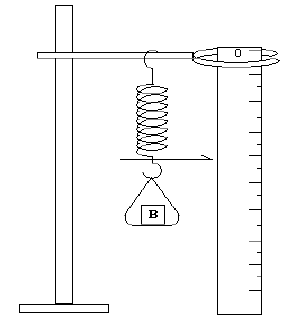
\includegraphics{./img/spring-practical.png}
\end{center}

\begin{enumerate}
\item{Set up the apparatus as shown with the zero mark of the meter-rule at the top
of the rule and record the scale reading, as shown by the pointer, $S_0$.}
\item{Place the object $B$ and standard weight (mass) $W$ equal to 20~g in the pan
and record the new pointer reading, $S_1$. Calculate the extension, $e = S_1 - S_0$ in
cm.}
\item{Repeat the procedure above with $W$ = 40~g, 60~g, 80~g and 100~g.}
\item{Record your results in tabular form as shown below:

\begin{center}
\begin{tabular}{ | c | c | c | c | c | }
\hline
$S_0$ & Mass (kg) & Force, $F$ (N) & Pointer Reading $S_1$ (cm) & Extension, $e = S_1 - S_0$ (cm) \\ \hline
& 0 & & & \\ \hline
& 0.02 & & & \\ \hline
& 0.04 & & & \\ \hline
& 0.06 & & & \\ \hline
& 0.08 & & & \\ \hline
& 0.1 & & & \\ \hline
\end{tabular}
\end{center}

}%Record your results...
\item{Plot a graph of force $F$ (vertical axis) against extension $e$ (horizontal axis).}
\item{Use your graph to evaluate
\begin{enumerate}
\item{mass of $B$}
\item{spring constant, $K$, given that the force, extension, constant and
weight of $B$ are related as follows: $$F = Ke - B$$}
\end{enumerate}
}%Use your graph...
\end{enumerate}

\subsubsection{Discussion}

This practical has two parts: the first is to find the spring constant $k$, the second is
to find the mass of an unknown object $B$. By looking at the equation above, we
can see that $F$ is the dependent variable, $e$ is the independent variable, $K$ is the slope and
$-B$ is the intercept. When the graph is drawn, $K$ and $B$ can be found easily. Note that the
intercept on the graph will be negative.

The procedure is simply to start from a certain point on the metre rule (it does not
need to be a specific number) and to add masses one at a time, measuring the distance
from your starting point to the new position. This distance is called the extension, $e$. Be
sure that you are not simply reading the metre rule, but are measuring the distance from
the starting point.

\subsection{Simple Pendulum (Form 2)}

With some practice, this experiment should be simple for anyone to perform. The
trick comes with the math and graphing (again, an example is shown below). The
materials can all be local (string, stones, ruler) except for the stopwatches (for which you
should consult the materials section).

The practical usually has one objective: to find the acceleration due to gravity, $g$.
We know that the mass of a pendulum and its angle of deflection (for small angles) do
not affect its period. Therefore we vary only the length $L$ of the pendulum and measure
its period, as shown in the following example question.

\subsubsection{Practical Sample Question}

The aim of this experiment is to determine the magnitude of the acceleration due to
gravity, $g$. Proceed as follows:

\begin{center}
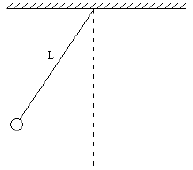
\includegraphics{./img/pendulum.png}
\end{center}


\begin{enumerate}
\item{Make a simple pendulum by suspending a weight on a string 10~cm long from a retort
stand.}
\item{Allow the pendulum to swing for twenty oscillations, using a stopwatch to record the
time. Repeat this procedure for pendulum lengths of 20~cm, 30~cm, 40~cm, and 50~cm.}
\item{Record your results in tabular form as shown below}

\begin{center}
\begin{tabular}{ | c | c | c | c | }
\hline
Pendulum Length l (m) & Time for 20 oscillations (s) & Period $T = \frac{t}{20}$ (s) & $T^2$ ($s^2$) \\ \hline
0.1 & & & \\ \hline
0.2 & & & \\ \hline
0.3 & & & \\ \hline
0.4 & & & \\ \hline
0.5 & & & \\ \hline
\end{tabular}
\end{center}

\item{Plot a graph of $T^2$ (vertical axis) against Pendulum Length (horizontal axis).}
\item{Calculate the slope of the graph.}
\item{Use the slope to calculate the value of $g$.}
\item{What are possible sources of error in this experiment?}

\end{enumerate}

\subsubsection{Discussion}

The period of a pendulum can be calculated using $$T = 2\pi\sqrt{\frac{l}{g}}$$
where $l$ is the length of the pendulum, $T$ is the period and $g$ is the acceleration due to
gravity. By squaring both sides, we get a much easier equation to graph: $$T^2 = 4\pi\frac{l}{g}$$ In this equation we see that $T^2$ is the dependent variable (y-axis) and $l$ is the
independent variable (x-axis), so the slope must be $$\mathrm{slope} = \frac{4\pi}{g}$$ 
When the graph is complete, the value of $g$ can be calculated easily.

Many students are confused by the difference between the time for many oscillations and
the period, which is the time for one oscillation. Be sure that they can change between
the two easily.

Note that pendulum practicals do not always require students to find $g$. Sometimes they are just required to find the relationship between $l$ and $t$. Again, it is essential that students read and understand the examination question, rather than memorize past solutions, and that they have lots of practice in collecting, organizing, and graphing data from a variety of experiments.

\subsection{Principle of Moments (Form 2)}

This experiment is used to verify the Principle of Moments, or equilibrium, by
balancing a meter rule on a knife-edge with masses at various distances. Usually the
students will need to calculate the mass of the meter rule. For this experiment, they need
a solid understanding of the Center of Gravity, the Moment of a force, and equilibrium.
No example question is given here, but the questions can range from asking for
the mass of the metre rule to finding the mass of an unknown object. They are all
variations on the same practical: using the condition of equilibrium to find mass.

\subsection{Finding the mass of a metre rule}

The mass of a uniform solid object, like a metre rule, is assumed to be at the
center of the object. In the case of the metre rule, we can say that the center of mass is at
the 50~cm mark, directly in the center. If we want it to be in equilibrium, the moments on
either side of a pivot must be equal, or $$ \mathrm{Clockwise moment} = \mathrm{Anticlockwise moment}$$
To find the mass of the metre rule itself, we begin by placing a known mass at one
point on the metre rule. We then move the pivot to one side or another until the metre
rule is perfectly balanced in equilibrium. As shown in the diagram below, the pivot will
not be at the 50~cm mark.

\begin{center}
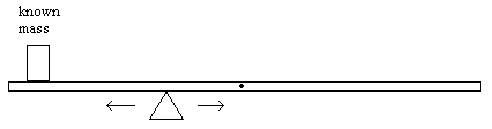
\includegraphics{./img/meter-rule.png}
\end{center}

If the metre rule is in equilibrium, we know that the moments must be equal, or
that $$F_{\mathrm{clockwise}} \times d_{\mathrm{clockwise}} = F_{\mathrm{anticlockwise}} \times d_{\mathrm{anticlockwise}}$$
In this case, the anticlockwise force is the weight of the object, and the distance is that
from the pivot to the object. The clockwise force is the weight of the metre rule, and the
distance is that from the 50~cm mark (center of mass) to the pivot. Therefore our
equation is: $$ W_{\mathrm{rule}} \times d_{\mathrm{rule}} = W_{\mathrm{object}} \times d_{\mathrm{object}} $$
Because the weight of the object is known, and the two distances can be measured, we
can easily calculate the mass and therefore the weight of the metre rule:
$$W_{\mathrm{rule}} = \frac{W_{\mathrm{object}} \times d_{\mathrm{object}}}{d_{\mathrm{rule}}}$$
From this we can calculate mass of the metre rule using $F = mg$.

Other questions follow the same rule of finding equilibrium and using the equal
moments to calculate an unknown mass. Be sure that you are familiar with calculating
moments and using the condition of equilibrium.

%==============================================================================
\section{Light}
The light practical always involves plane mirrors or glass blocks (rectangular
prisms). Presumably you will have already done these practicals with the students in Form
three (refraction) and Form 1 (plane mirrors), but a little practice will make the theory and
execution clear, especially if they can work in groups. The materials you will need are as
follows:
\begin{description}
\item[Cork Board]{Use cardboard for this, about 0.5 to 0.75~cm thick.}
\item[Optical pins]{Use sewing pins or syringe needles. If using syringe needs, be
sure to crimp the ends so students do not prick themselves.}
\item[Protractors]{These are cheap and students are supposed to have them anyway.
Small ones come in local mathematical sets.}
\item[Glass Block / Rectangular Prism]{A simple rectangular piece of 6~mm glass,
about 8~cm by 12~cm, will work.}
\item[Plane Mirror]{You can buy mirror glass in town in small sections for 200/= or
less; it should be available in villages through the local craftsmen if they work on
windows. Alternately, you can smoke one side of a piece of glass to make the
other side like a mirror.}
\end{description}

\subsection{Plane Mirror Practicals (Form 1)}

These are not as common as they are easy to fudge, but they come in a variety of
questions:
\begin{itemize}
\item{Placing pins in front of a mirror at different distances and finding the distance of
the image.}
\item{Verifying the Law of Reflection at plane mirrors.}
\item{Placing two mirrors at different relative angles to find the number of images
produced.}
\end{itemize}
These are not overly complicated, but practice with your students creating images in
mirrors -- they are not as accustomed to playing with mirrors as you might be.

\subsection{Rectangular Prism (Form 3)}

Students will be asked to find the refractive index of the glass block by varying
the angle of incidence $i$ and measuring the corresponding angles of refraction $r$ as
described in the Mathematics section earlier. They will do this by placing two pins in
front of the prism, which together form a `ray' (our light ray), and then placing two more
pins on the other side of the prism so that, when observed through the prism from either
side, the four pins line up exactly. By drawing the lines that the pins make on the paper,
the refracted ray inside the prism can be easily traced, and the refracted angle measured.
An example question is given below.

\subsubsection{Practical Sample Question}

The aim of this experiment is to find the refractive index of a glass block. Proceed
as follows:
\begin{enumerate}
\item{Place the given glass block in the middle of the drawing paper on the drawing
board. Draw lines along the upper and lower edges of the glass block. Remove the
glass block and extend the lines you have drawn. Represent the ends of these line
segments as $SS_1$ and $TT_1$. Draw the normal $NN_1$ to the parallel lines $SS_1$ and
$TT_1$ as shown in the figure below:

\begin{center}
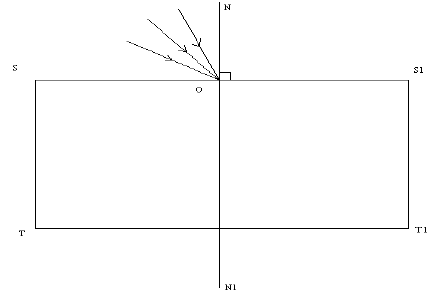
\includegraphics{./img/light-block-1.png}
\end{center}

}%Place the given...

\item{Draw five evenly spaced lines from O to represent incident rays at different
angles of incidence (10, 20, 30, 40, and 50 degrees from the normal). Replace the
glass block carefully between $SS_1$ and $TT_1$. Stick two pins $P_1$ and $P_2$ as shown in
the figure as far apart as possible along one of the lines drawn to represent an
incident ray. Locate an emergent ray by looking through the block and stick pins
$P_3$ and $P_4$ exactly in line with images $I_1$ and $I_2$ of pins $P_1$ and $P_2$. Draw the
emergent ray and repeat the procedure for all the incident rays you have drawn.}
\item{Finally draw the corresponding refracted rays.}

\begin{center}
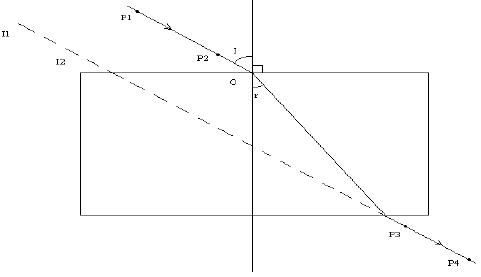
\includegraphics{./img/light-block-2.png}
\end{center}

\item{Record the angles of incidence $i$ and the measured corresponding angles of
refraction $r$ in a table. Your table of results should include the values of
$\sin{i}$ and $\sin{r}$.}
\item{Plot the graph of $\sin{i}$ (vertical axis) against $\sin{r}$ (horizontal axis).}
\item{Determine the slope of the graph.}
\item{What is the refractive index of the glass block used?}
\item{Mention any sources of errors in this experiment.}
\end{enumerate}

\subsubsection{Discussion}

In this experiment, pins are used to simulate a ray of light. If all of the pins are
aligned as you look through the block, they act as a single ray. It takes practice to be able
to align the pins while looking through the block, so practice often with your students.

Light slows down as it enters a denser medium, so in order to minimize the time
required to pass through that medium, it changes direction until it moves back into its
original medium. In this case, light is moving from air into glass and then back into air,
so its direction changes while inside the glass, then returns to its original direction when
passing back into air. This effect is called refraction and it depends on the nature of the
media, in this case air and glass. Snell’s law gives us the relationship between the nature
of the media and the resulting angles of incidence and refraction:
$$n_1 \times \sin{i} = n_2 \times \sin{r}$$

In this experiment, the incident angle $i$ is being changed and the refracted angle $r$
is being measured. The refractive index of medium 1 (air) is known as 1.0, so we can use
these three to find the refractive index of medium 2 (glass). On the graph, $\sin{i}$ is the
dependent variable and $\sin{r}$ is the independent variable, so the equation becomes
$$\sin{i} = 2 \sin{r} \frac{n_2}{n_1}$$
In this case the slope must be $\frac{n_2}{n_1}$

The refractive index of medium air is simply 1.0, so the slope is the refractive index of
medium 2.

This practical is one of the easiest to perform with students because it does not
require any preparation. Syringe needles should be readily available and glass blocks are
cheap, so it is possible to have every students try this themselves many times before
taking the exam.

%==============================================================================
\section{Electricity}

This is by far the least attempted practical on the exam, but not because it is
difficult. The electricity practical, if properly set up, is one of the easiest to perform. It
can appear in many different forms but will always involve a simple circuit and some
kind of variable resistor in order to measure current or EMF for different resistances. The
materials you will probably need are as follows:

\begin{description}
\item[Connecting wires]{Use speaker wire; it is cheap and available in most villages
and towns.}
\item[Voltmeters, Ammeters, Galvanometers]{This is unavoidable; you can get full
digital multimeters in town for about 10,000/=, galvanometers can be found in
any lab store or can be made using a compass and insulated copper wire.}
\item[Batteries]{Two D-size batteries should easily be enough for this experiment.}
\item[Spools of wires of various diameters]{These are used to make small resistors for
the metre bridge or potentiometer. The most common type of wire to use is
nichrome, which can be found in a hardware store. Steel will also work, though it
is less resistant and therefore harder to measure.}
\item[Metre Bridges]{See the activity that describes the construction of a metre bridge
and potentiometer. It is best to make both together as the construction is almost
identical and both are used frequently.}
\item[Variable Resistor (rheostat)]{This is optional as it is typically only used to set a
level that can be easily read by the voltmeter. However, if you are using a
multimeter, you can simply change the magnitude setting on the multimeter to
account for unusually low or high resistances.}
\end{description}

\subsection{Potentiometers}

This experiment is very simple but requires the correct materials, namely the
meter bridge/potentiometer described above. A complete circuit is created with a switch
(optional), power source, variable resistor and 1~m of bare resistance wire, all in series.

The potentiometer itself is simple to construct; all preparation is done by the teacher, so
the student simply follows the instructions as shown in the following example.

\subsubsection{Practical Sample Question}

The aim of this experiment is to determine the potential fall along a uniform
resistance wire carrying a steady current. Proceed as follows:

\begin{center}
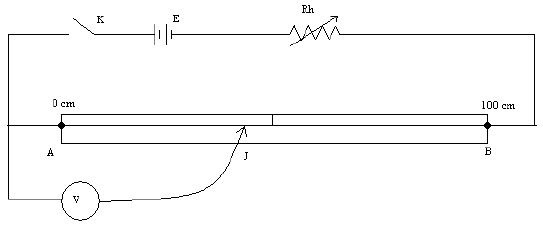
\includegraphics{./img/meter-bridge-1.png}
\end{center}

\begin{enumerate}
\item{Connect up the circuit as shown in the figure. Adjust the rheostat so that when the sliding
contact J is near B and the key is closed the voltmeter V indicates an almost full scale
of deflection. Do not alter the rheostat again.}
\item{Close key K and make contact with J, so that AJ = 10~cm. Record the potential
difference V volts between A and J as registered on the voltmeter.}
\item{Repeat this procedure for AJ = 20~cm, 30~cm, 50~cm, and 70~cm.}
\item{Tabulate your results for the values of AJ and V.}
\item{Plot a graph of V (vertical axis) against AJ (horizontal axis).}
\item{Calculate the slope of the graph.}
\item{What is your comment on the slope?}
\item{State any precautions on the experiment.}
\end{enumerate}

\subsubsection{Discussion}

This is a simple test of the relationship between the length of a wire and its
resistance, which we know is $$R=\frac{\rho l}{A} $$

Where $l$ is the length of the wire, $\rho$ is the nature of the wire, and $A$ is the cross-sectional
area of the wire. We expect that as the length of wire increases, its potential difference
will also increase because the resistance (and therefore potential difference) of a wire is
directly related to its length. The voltmeter in this experiment is measuring just the
potential difference over the length of wire (10~cm, 20~cm, etc.); if we use Ohm’s Law to say that $V = IR$, we can write:\\
$$ V = \frac{I \rho l}{A} $$
In this experiment, $I$, $\rho$ and $A$ are all constant, so the slope is
$$\mathrm{slope} = \frac{I \rho}{A} $$
and we can find the resistivity, $\rho$, though it is not asked for directly in the question.

\subsection{Metre Bridges}

A metre bridge resembles a potentiometer, except that it uses a galvanometer to
measure the difference in current between two points on the circuit, hence the name
``bridge.'' The same materials can be used as with the potentiometer, though it is best to
use small coils of resistance wire for the small resistors (between 3$\Omega$ and 20$\Omega$ is a good resistance). A galvanometer can be made easily if one is not available.

\begin{center}
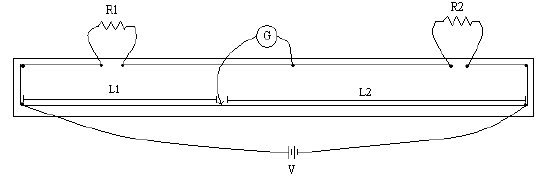
\includegraphics{./img/meter-bridge-2.png}
\end{center}

Resistors $R_1$ and $R_2$ have different resistances, but they should be somehow similar so
that one resistors does not take all of the current (this will make it difficult to measure the
length to the galvanometer). About 5$\Omega$ and 10$\Omega$, for example, would work well.

However, for the sake of the practical, one resistor should not be known; the objective of
the practical is to find the unknown resistance. The long wire along the bottom edge is a
metre of nichrome wire or other resistance wire. One terminal of the galvanometer is
connected between the two resistors, and the other terminal is connected to a flying wire
that is free to move along the length of the nichrome wire.

The practical instructs you to move the galvanometer's flying wire back and forth
along the nichrome wire until it reads zero. At this point, we know that no current is
passing through the galvanometer, so the potential difference across it is zero. This
means that the current flowing through $R_1$ is the same as that current flowing through $R_2$,
and the current flowing through the nichrome wire is constant. From this we can
conclude that
$$ \frac{R_1}{L_1} = \frac{R_2}{L_2} $$
or that the ratio of the two resistors is equal to the ratio of distances from the flying wire
to either end of the nichrome wire. The resistance of one resistor (say, $R_1$) is known and
the lengths $L_1$ and $L_2$ can be measured from the flying wire to either side of the
nichrome wire. Using the ratio above, we can easily calculate the unknown resistance $R_2$.

\subsection{Ohm’s Law (Form 2)}

The practical may give any kind of experiment to use or verify Ohm’s Law in a
simple circuit. Internal resistance of cells appears frequently. Be sure that your students
understand every part of the law and can find their way around a simple circuit. When
graphing, the internal resistance of a cell appears as the y-intercept.

The more familiar your students are with these techniques, the better they will do.
Perform these practicals as often as possible: when the topic comes up, when preparing
for the mock and NECTA exams, and any time you can get them to come in for an
evening session or a weekend. They will make many, many mistakes the first couple of
times through but that is exactly what you want as they will learn from their mistakes and
remember them.
